\documentclass[tikz,border=3.14mm]{standalone}

\def\height{1}
\definecolor{darkgray}{HTML}{373737}
\definecolor{lightgray}{HTML}{b0b0b0}
\definecolor{lpurple}{HTML}{ffffff}
\definecolor{dpurple}{HTML}{434752}
\definecolor{jkfs}{HTML}{e1e9ef}
\begin{document}
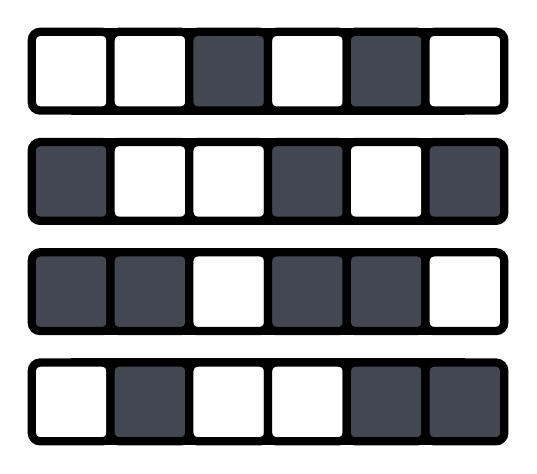
\begin{tikzpicture}[node distance=2.5cm, >=stealth]

\draw[fill=lpurple, line width=3, rounded corners=3] (0,0) rectangle (1,-\height);
\node at (0.5, -0.5) {};

\draw[fill=lpurple, line width=3, rounded corners=3] (1,0) rectangle (2,-\height);
\node at (1.5, -0.5) {};
\draw[fill=dpurple, line width=3, rounded corners=3] (2,0) rectangle (3,-\height);
\node at (2.5, -0.53) {};
\draw[fill=lpurple, line width=3, rounded corners=3] (3,0) rectangle (4,-\height);
\node at (3.5, -0.5) {};
\draw[fill=dpurple, line width=3, rounded corners=3] (4,0) rectangle (5,-\height);
\node at (4.5, -0.53) {};
\draw[fill=lpurple, line width=3, rounded corners=3] (5,0) rectangle (6,-\height);
\node at (5.5, -0.5) {};


\draw[fill=dpurple, line width=3, rounded corners=3] (0,-1.4) rectangle (1,-1.4-\height);
\node at (0.5, -1.93) {};
\draw[fill=lpurple, line width=3, rounded corners=3] (1,-1.4) rectangle (2,-1.4-\height);
\node at (1.5, -1.9) {};
\draw[fill=lpurple, line width=3, rounded corners=3] (2,-1.4) rectangle (3,-1.4-\height);
\node at (2.5, -1.95) {};
\draw[fill=dpurple, line width=3, rounded corners=3] (3,-1.4) rectangle (4,-1.4-\height);
\node at (3.5, -1.93) {};
\draw[fill=lpurple, line width=3, rounded corners=3] (4,-1.4) rectangle (5,-1.4-\height);
\node at (4.5, -1.9) {};
\draw[fill=dpurple, line width=3, rounded corners=3] (5,-1.4) rectangle (6,-1.4-\height);
\node at (5.5, -1.93) {};

\draw[fill=dpurple, line width=3, rounded corners=3] (0,-2.8) rectangle (1,-2.8-\height);
\node at (0.5, -3.33) {};
\draw[fill=dpurple, line width=3, rounded corners=3] (1,-2.8) rectangle (2,-2.8-\height);
\node at (1.5, -3.33) {};
\draw[fill=lpurple, line width=3, rounded corners=3] (2,-2.8) rectangle (3,-2.8-\height);
\node at (2.5, -3.35) {};
\draw[fill=dpurple, line width=3, rounded corners=3] (3,-2.8) rectangle (4,-2.8-\height);
\node at (3.5, -3.33) {};
\draw[fill=dpurple, line width=3, rounded corners=3] (4,-2.8) rectangle (5,-2.8-\height);
\node at (4.5, -3.33) {};
\draw[fill=lpurple, line width=3, rounded corners=3] (5,-2.8) rectangle (6,-2.8-\height);
\node at (5.5, -3.3) {};

\draw[fill=lpurple, line width=3, rounded corners=3] (0,-4.2) rectangle (1,-4.2-\height);
\node at (0.5, -4.7) {};
\draw[fill=dpurple, line width=3, rounded corners=3] (1,-4.2) rectangle (2,-4.2-\height);
\node at (1.5, -4.73) {};
\draw[fill=lpurple, line width=3, rounded corners=3] (2,-4.2) rectangle (3,-4.2-\height);
\node at (2.5, -4.73) {};
\draw[fill=lpurple, line width=3, rounded corners=3] (3,-4.2) rectangle (4,-4.2-\height);
\node at (3.5, -4.7) {};
\draw[fill=dpurple, line width=3, rounded corners=3] (4,-4.2) rectangle (5,-4.2-\height);
\node at (4.5, -4.73) {};
\draw[fill=dpurple, line width=3, rounded corners=3] (5,-4.2) rectangle (6,-4.2-\height);
\node at (5.5, -4.73) {};

\draw[fill=black] (0.5,0.0456) rectangle (5.5,-.03);
\draw[fill=black] (0.5,-.97) rectangle (5.5,-1.0456);
\draw[fill=black] (0.5,0.0456-2.8) rectangle (5.5,-.03-2.8);
\draw[fill=black] (0.5,-.97-2.8) rectangle (5.5,-1.0456-2.8);
\draw[fill=black] (0.5,0.0456-1.4) rectangle (5.5,-.03-1.4);
\draw[fill=black] (0.5,-.97-1.4) rectangle (5.5,-1.0456-1.4);
\draw[fill=black] (0.5,0.0456-4.2) rectangle (5.5,-.03-4.2);
\draw[fill=black] (0.5,-.97-4.2) rectangle (5.5,-1.0456-4.2);
\end{tikzpicture}
\end{document}